\subsubsectionwithauthor[author={Mika Landeck},email={mika.landeck@fau.de}]{Aufgabe 3: Chomsky-Hierarchie}

\paragraph{(a)}
	$L_1 = \{ w \in L: vor\ jedem\ (\ stehen\ mehr\ [\ als\ ] \}$ 
	
	\begin{quote}
		\textbf{Pumpinglemma für kontextfreie Sprachen} \\
		Ist $L$ eine kontextfreie Sprache, so gilt: \\
		$\exists p \in \mathbb{N}: \forall z \in L, |z| \geq p:$ \\
		$\exists u,v,w,x,y \in \Sigma^*: z = uvwxy$ mit
		\begin{enumerate}
			\item $|vx| \geq 1$
			\item $|vwx| \leq p$
			\item $\forall i \in \mathbb{N} : uv^{i}wx^{i}y \in L$
		\end{enumerate}
	\end{quote}

	Nehmen wir an $L_1$ sei kontextfrei, dann können wir das Pumpinglemma anwenden und folgern:
	
	Sei $p \in \mathbb{N}$ die Pumpingzahl. Wir wählen $z = [^p(]^p)] \in L_1$ mit $|z| = 2p+2 > p$.\\
	Aus $|vwx| \leq p$ und $|vx| \geq 1$ ergeben sich für die Form von $vwx$ folgende Fälle:
	\begin{enumerate}
		\item $v=[^k$ und $x=[^l$ mit $p \geq k+l  \geq 1$
		\item $v=[^k$ und $x=[^l(]^m$ mit $p-1 \geq k+l+m  \geq 0$
		\item $v=[^k(]^l$ und $x=]^m$ mit $p-1 \geq k+l+m  \geq 0$
		\item $v=]^l$ und $x=]^m$ mit $p \geq l+m  \geq 1$
		\item $v=]^l$ und $x=]^m)$ mit $p-1 \geq l+m  \geq 0$
	\end{enumerate}

	In Fall 1 ist $uv^2wx^2y=[^{p+k+l}(]^{p}) \notin L_1$, da $p+k+l > p$ und somit liegt keine korrekte Klammerung mehr vor.\\
	In Fall 2 ist $uv^2wx^2y=[^{p+k}(]^{m}[^{l}(]^{p}) \notin L_1$, da zwei $($ und nur eine $)$ vorkommen. Somit liegt keine korrekte Klammerung vor.\\
	In Fall 3 ist $uv^2wx^2y=[^{p}(]^{l}[^{k}(]^{p+m}) \notin L_1$, da zwei $($ und nur eine $)$ vorkommen. Somit liegt keine korrekte Klammerung vor.\\
	In Fall 4 ist $uv^2wx^2y=[^{p}(]^{p+l+m}) \notin L_1$, da $p+l+m > p$ und somit liegt keine korrekte Klammerung mehr vor.\\
	In Fall 5 ist $uv^2wx^2y=[^{p}(]^{p+l})]^{m}) \notin L_1$, da zwei $)$ und nur eine $($ vorkommen. Somit liegt keine korrekte Klammerung vor.
	
	Das ist ein Widerspruch zur Annahme $L_1$ sei kontextfrei. $\Rightarrow L_1$ ist nicht kontextfrei $\Rightarrow L_1$ ist nicht regulär, da die regulären Sprachen eine Teilmenge der kontextfreien Sprachen bilden. 

	\vspace{0.3cm}
\paragraph{(b)}
	$L_2 = \{ w \in L: auf\ jede\ \ddot{o}ffnende\ Klammer\ folgt\ direkt\ eine\ schließende\ Klammer \}$
	
	Zu $L_2$ lässt sich folgender DEA bauen, der sie akzeptiert:
	\begin{center}
		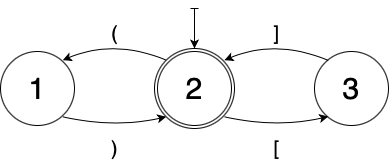
\includegraphics[scale=0.5]{DEA zu Klammersprache.png}	
	\end{center}
	
	Somit ist $L_2$ regulär und damit auch kontextfrei, denn die regulären Sprachen sind eine Teilmenge der kontextfreien Sprachen.
	